\documentclass[12pt]{article}

\usepackage{graphicx}
\usepackage{geometry}
\usepackage{amsmath}
\geometry{margin=1in}

\begin{document}

% ---------------- LOGO ----------------
\begin{center}

\includegraphics[width=6cm]{iiitb_logo.jpg}

\vspace{0.3cm}

\Large \textbf{IIITB COMET FOUNDATION}
\end{center}

\vspace{0.5cm}

\noindent
\textbf{Name:} Anushree M R\\
\textbf{Id:} COMETFWC063

\vspace{0.5cm}

\begin{center}
\Large \textbf{GATE Question No. 31}
\end{center}

% ---------------- QUESTION ----------------
\section*{Question}

\begin{center}
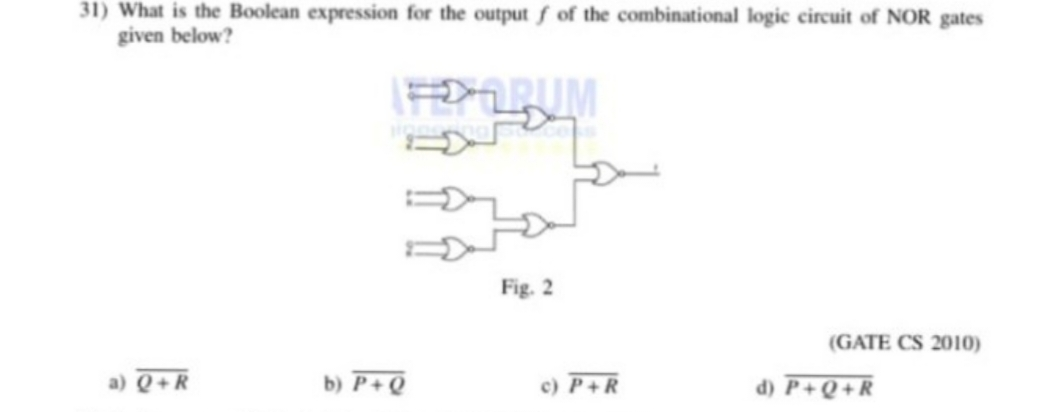
\includegraphics[width=0.8\textwidth]{Screenshot_20260224_115343.jpg}
\end{center}

The Boolean expression for the output of the combinational logic circuit using NOR gates is to be implemented.

% ---------------- ANALYSIS ----------------
\section*{Question Analysis}

The given circuit consists only of NOR gates.

Using NOR properties:

\[
f = \overline{P + Q + R}
\]

This represents a 3-input NOR gate.

% ---------------- TRUTH TABLE ----------------
\section*{Truth Table}

\begin{center}
\begin{tabular}{|c|c|c|c|}
\hline
P & Q & R & f \\
\hline
0 & 0 & 0 & 1 \\
0 & 0 & 1 & 0 \\
0 & 1 & 0 & 0 \\
0 & 1 & 1 & 0 \\
1 & 0 & 0 & 0 \\
1 & 0 & 1 & 0 \\
1 & 1 & 0 & 0 \\
1 & 1 & 1 & 0 \\
\hline
\end{tabular}
\end{center}

% ---------------- LOGIC DESCRIPTION ----------------
\section*{Logic Description}

Inputs $P$, $Q$, and $R$ are applied to NOR logic.

\[
f = \overline{P + Q + R}
\]

Output becomes HIGH only when all inputs are LOW.

% ---------------- CONCLUSION ----------------
\section*{Conclusion}

The NOR logic circuit successfully implements a 3-input NOR gate and the obtained results match the theoretical truth table.

\end{document}
